\section{Experiments}
\label{sec:experiments}

% fix algorithm shortcuts, add greedy and brute to the supplement
We compare \tsip~ and \greedy~ on the Iris and Wine datasets \citep{misc_iris_53, misc_wine_109, scikit-learn}, as well as the Ethanol dataset from \citet{Chmiela2018-at, Koelle2022-ju}.
The latter is an interpretability dataset where a dictionary of interpretable features are evaluated for their ability to parameterize the data manifold through computation of their Jacoban matrices and projection onto estimated tangent spaces (see \citet{Koelle2022-ju} for preprocessing details).
Statistical replicas for Wine and Iris are created by resampling across $P$, while for Ethanol they are created by sampling from different points on the data manifold.
For basis pursuit, We use the SCS interior point solver \citep{ocpb:16} from CVXPY \citep{diamond2016cvxpy, agrawal2018rewriting}, which is able to push sparse values arbitrarily close to 0 \citep{cvxpy_sparse_solution}.

\begin{figure}[h]
\centering
\subcaptionbox{Boxplot of $\widehat S_{g}$. \label{fig:boxplot1}}
{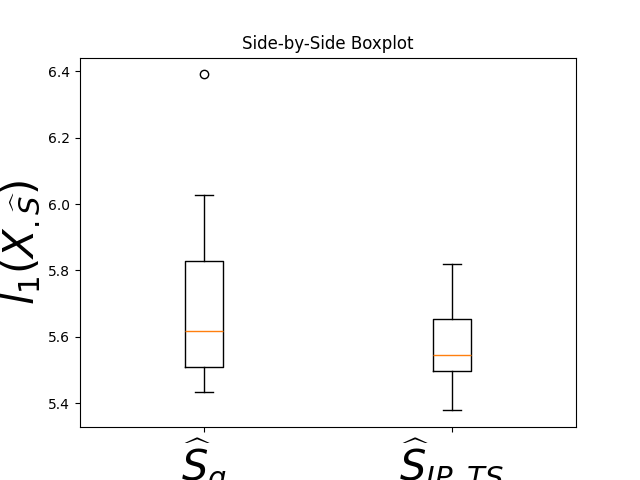
\includegraphics[width=.3\textwidth]{/Users/samsonkoelle/convexlocalisometry/figures/Figure2b.png}}
\subcaptionbox{Boxplot of $\widehat S_{TS}$. \label{fig:boxplot2}}
{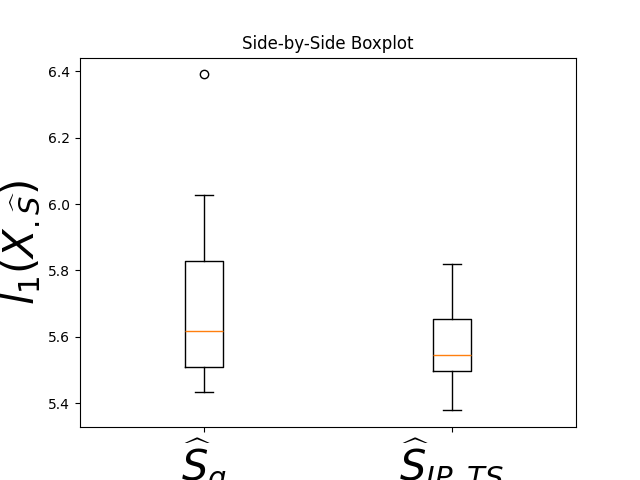
\includegraphics[width=.3\textwidth]{/Users/samsonkoelle/convexlocalisometry/figures/Figure2b.png}}
\subcaptionbox{Boxplot of $\widehat S_{third}$. \label{fig:boxplot3}}
{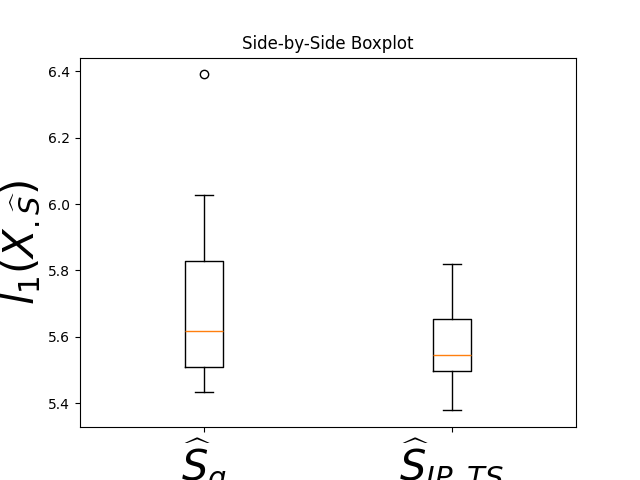
\includegraphics[width=.3\textwidth]{/Users/samsonkoelle/convexlocalisometry/figures/Figure2b.png}}
\caption{Comparison with isometry loss.}
\label{fig:boxplots}
\end{figure}

\begin{table}[h!]
\centering
\begin{tabular}{c|c|c|c|c|c|}
\hline
Name & $D$ & $P$ & $n$ & $I$ & $|\widehat{\mathcal{S}_1}|$ \\ \hline
% Add your data here
Iris & 1 & 2 & 3 & 4 & 5 \\ \hline
Wine & 6 & 7 & 8 & 9 & 10 \\ \hline
Ethanol & 11 & 12 & 13 & 14 & 15 \\ \hline
\end{tabular}
\caption{Experimental parameters and results.
For the Wine dataset, even \brute~ on $\widehat {\mathcal S}_1$ is prohibitive in $D=13$, and so we truncate our inputs to $D=5$.}
\label{tab:sample}
\end{table}